Navrhněte pravidla pro oboustranný převod mezi oběma formami ve spisovné češtině.


\section{First-person to Third-person Rules}
In First-person $\rightarrow$ Third-person conversion direction, I have proposed four rules. These four rules cover:
	\begin{itemize}
		\item Personal pronouns replacement
		\item Possesive pronouns replacement
		\item Replacement of contidional, present and future verb forms, conjunctions
		\item Auxiliary verbs replacement or deletion
	\end{itemize}

In this section, I describe each of these rules.

\subsection{Personal pronouns}

This rule covers the conversion of a personal pronoun \emph{já (I)} and its forms. The pronoun can be replaced by:
	\begin{itemize}
		\item another pronoun -- \emph{ona (she)}/\emph{on (he)}
		\item noun -- usually a proper noun, given as the protagonist's name
	\end{itemize}

In both cases, the replacement must be in a corresponding form to keep a sentence grammatically correct.

The rule is illustrated in a diagram \ref{fig:icher-perspron-rule}.

\begin{figure}[!htbp]
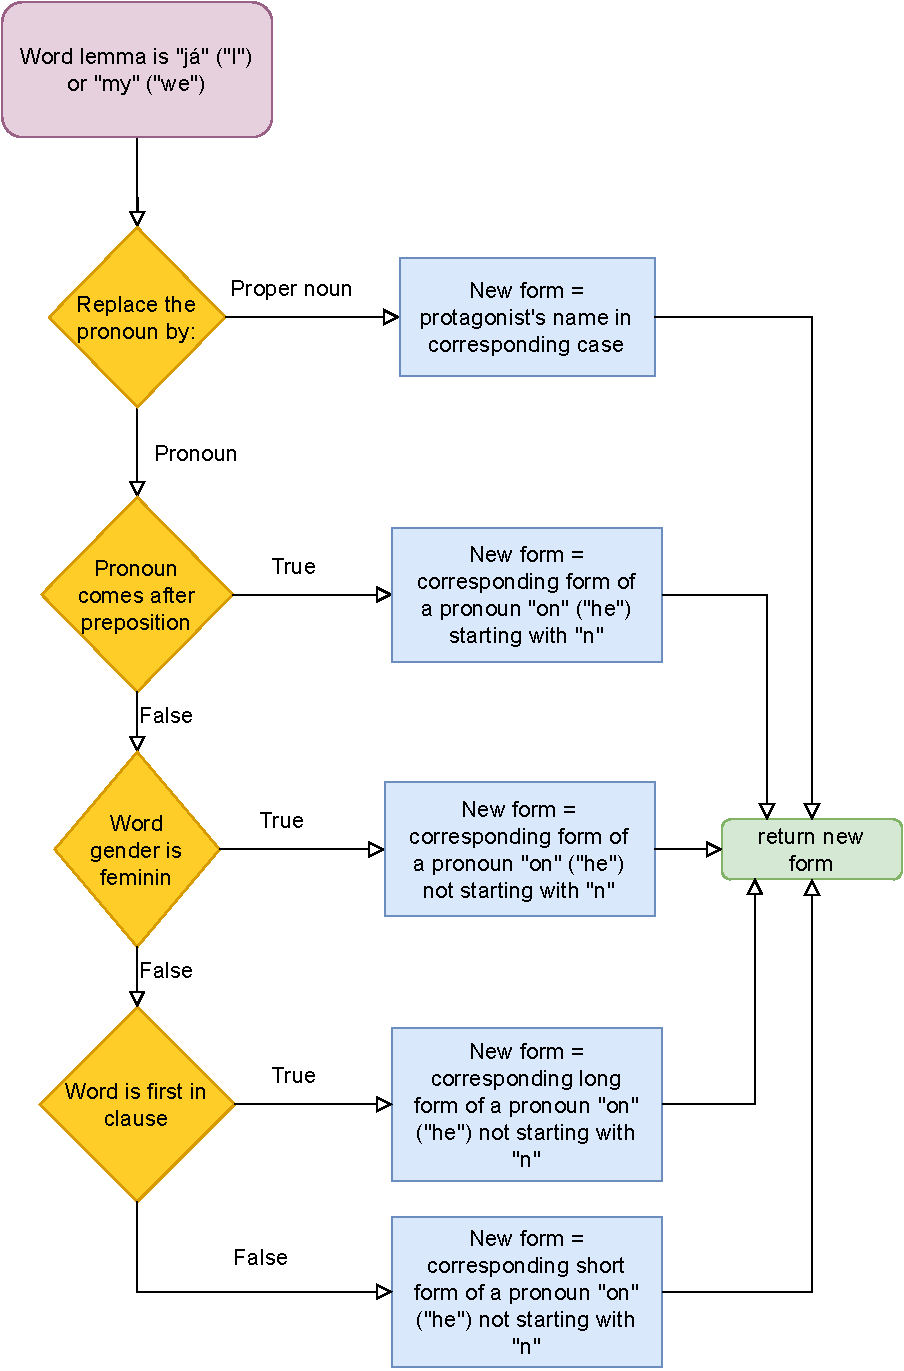
\includegraphics[width=\textwidth]{data/Icher-Perspron-Rule.pdf}
\caption{Personal pronouns replacement rule}
\label{fig:icher-perspron-rule}
\end{figure}

\subsection{Possessive pronouns}

In addition to personal pronouns, possessive pronouns must also be converted. The process is similar to the previous one. The goal is to convert a possessive pronoun \emph{můj (my)} and its forms to possessive pronouns \emph{její (her)} / \emph{jeho (his)}, or the possessive form of a proper noun. Considering the limits given by the morphological analyzer, I have decided not to include the second type of replacement. Therefore all the possessive pronouns would be replaced by possessive pronouns.

The rule is illustrated in a diagram \ref{fig:icher-posspron-rule}.

\begin{figure}[!htbp]
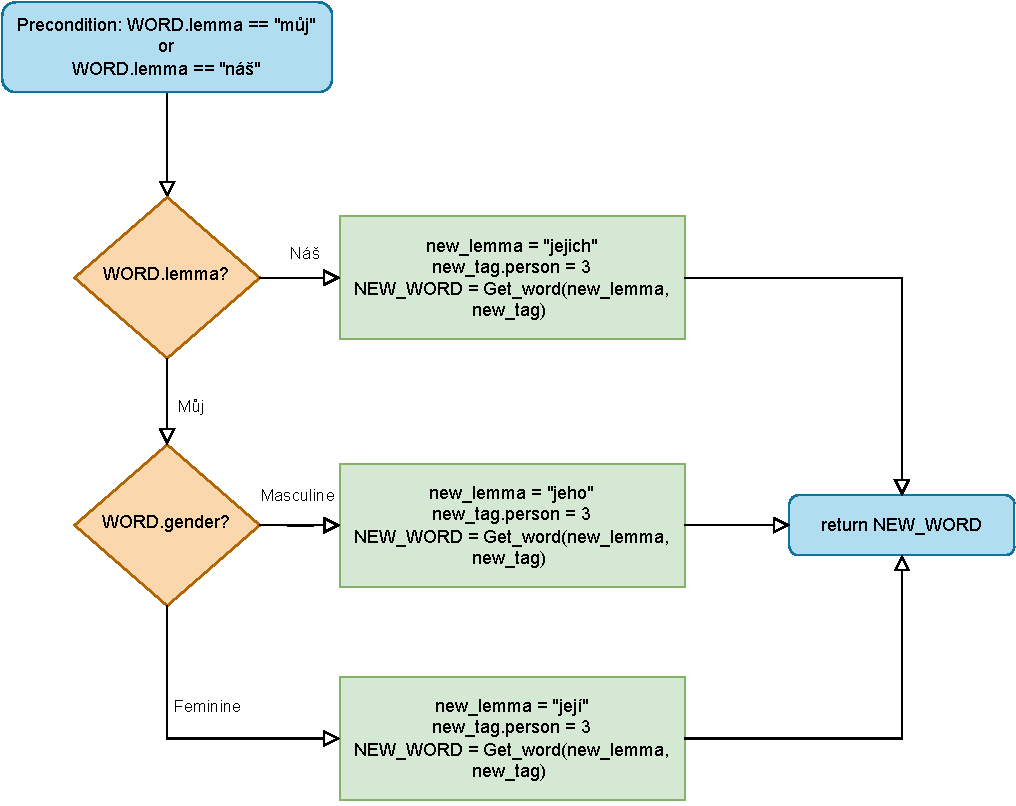
\includegraphics[width=\textwidth]{data/Icher-Posspron-Rule.pdf}
\caption{Possessive pronouns replacement rule}
\label{fig:icher-posspron-rule}
\end{figure}

\subsection{Conditionals, indicatives, conjunctions}

The third rule covers several cases because the conversion procedure is the same in all cases. The process is simple: we need to change the person in the word's tag and then generate a new word form from this new tag and the original lemma, as shown in \ref{fig:icher-predicate-rule}.

To put it simply, this rule includes these types of conversion:
\begin{itemize}
	\item bych/bychom $\rightarrow$ by -- \emph{conditional auxiliary verbs}
	\item budu/budeme $\rightarrow$ bude/budou -- \emph{future indicatives}
	\item píšu/píšeme $\rightarrow$ píše/píšeme -- \emph{example of present indicative}
	\item abych/abychom/kdybych/kdybychom $\rightarrow$ aby/kdyby -- \emph{conjunctions}
\end{itemize}


\begin{figure}[!htbp]
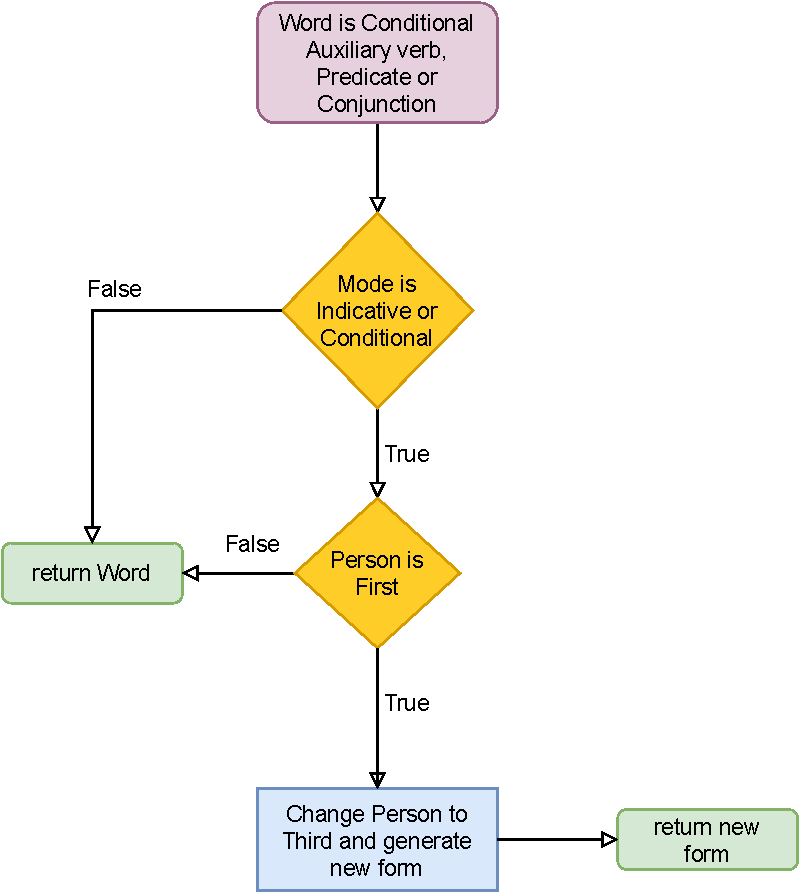
\includegraphics[width=\textwidth]{data/Icher-Predicate-Rule.pdf}
\caption{Rule replacing the conditionals, conjunctions and verb forms in present indicative tense and future indicative tense}
\label{fig:icher-predicate-rule}
\end{figure}

\subsection{Auxiliary verbs}

Finally, we need to replace or delete other auxiliary verbs. If the auxiliary verb depends on an active participle, the auxiliar should be deleted. However, if the participle is passive, the auxiliar should be kept and converted.

For example, a sentence \emph{Ukradl \textbf{jsem} klávesnici (I stole a keyboard)} converts to \emph{Ukradl klávesnici (He stole a keyboard)}, but \emph{\textbf{Jsem} ukradena (I am stolen)} should convert to \emph{\textbf{Je} ukradena (She is stolen)}.

Also, the auxiliary verb needs to be in the indicative mode to be converted. The conditional verbs are covered in the previous rule. Then, other modes of auxiliary verbs should not be converted at all, as the auxiliar in plusquamperfect. For instance, a sentence \emph{\textbf{Byl jsem} ukradl klávesnici} might convert to \emph{Juraj \textbf{byl} ukradl klávesnici}. As we can see, the sentence in the first-person narrative contains two auxiliary verbs; however, only the one in indicative mode would be deleted.

I present the rule in \ref{fig:icher-auxverb-rule}.

\begin{figure}[!htbp]
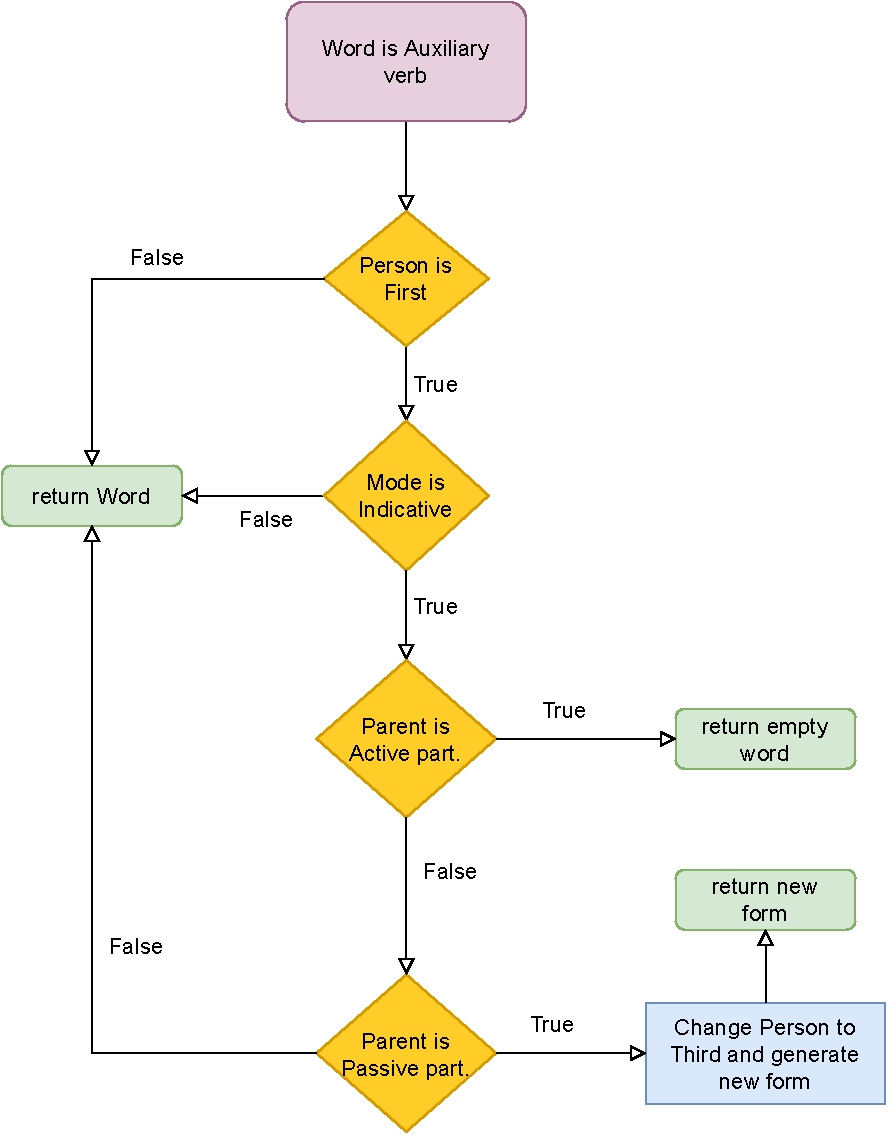
\includegraphics[width=\textwidth]{data/Icher-Auxverb-Rule.pdf}
\caption{Rule replacing the indicative forms of auxiliary verbs}
\label{fig:icher-auxverb-rule}
\end{figure}

\section{Third-person to First-person Rules}

Since this direction is much more complicated for conversion than the other one, I propose seven rules which cover:

\begin{itemize}
	\item Proper nouns replacement
	\item Predicates replacement
	\item Conditional auxiliars replacement
	\item Auxiliary verbs addition
	\item Personal pronouns replacement
	\item Possessive pronouns replacement
	\item Conjunction replacement
\end{itemize}

\subsection{Proper nouns}

The first rule deals with the occurrences of the protagonist's name. Firstly, we need to decide if we should replace the name with a personal pronoun or skip it. The name can only be skipped if the member is a subject and the name is not part of multiple subject coordination.

The rule is illustrated in figure \ref{fig:erich-name-rule}.

\begin{figure}[!htbp]
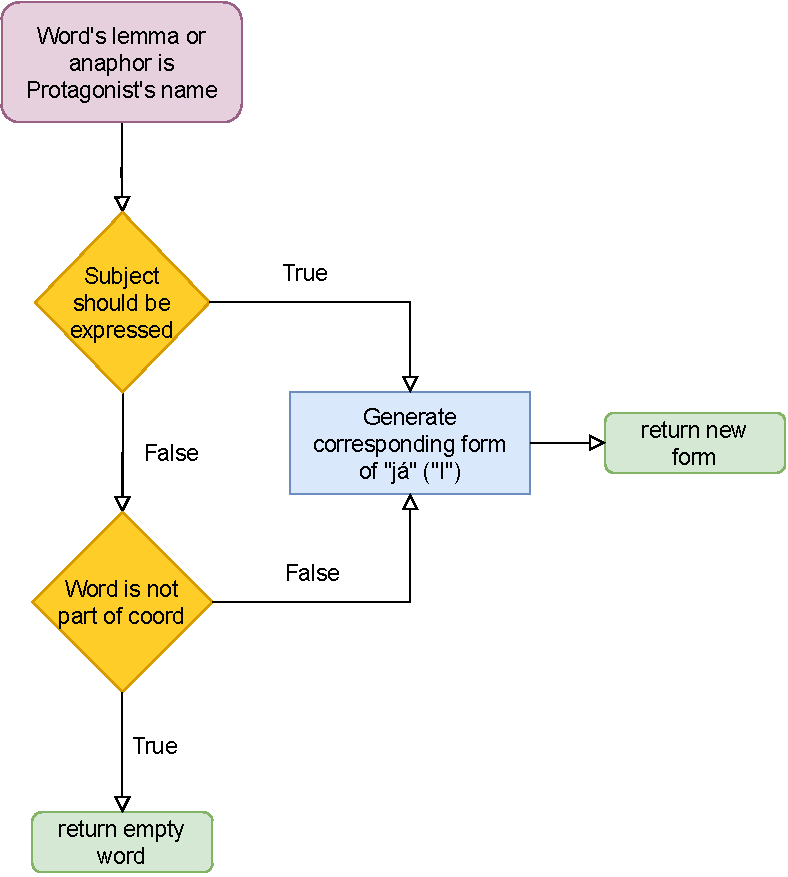
\includegraphics[width=\textwidth]{data/Erich-Name-Rule.pdf}
\caption{Rule replacing or skipping the occurrances of protagonist's name}
\label{fig:erich-name-rule}
\end{figure}

\subsection{Predicates}

Indicative verbs should be replaced. In contrast to First-person $\rightarrow$ Third-person conversion, the information about a person is not enough. We need to know the subject to our predicate and replace the word with a new form only if the subject refers to the protagonist, as I show in figure \ref{fig:erich-predicate-rule}

\begin{figure}[!htbp]
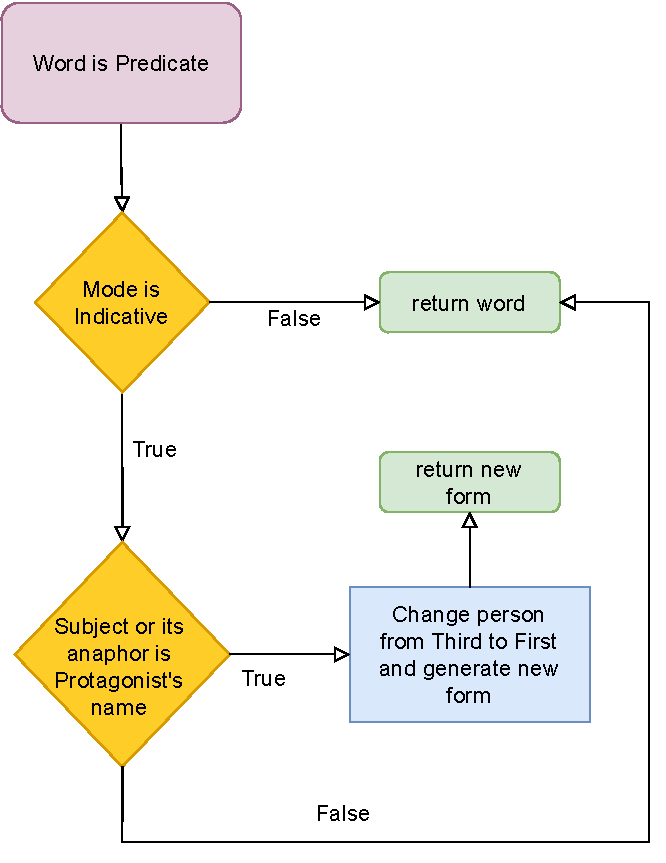
\includegraphics[]{data/Erich-Predicate-Rule.pdf}
\caption{Rule covering the predicate replacement}
\label{fig:erich-predicate-rule}
\end{figure}

\subsection{Conditional auxiliars}

These auxiliars are treated similarly to the predicates. I illustrate the decision process in figure \ref{fig:erich-conditional-rule}


\begin{figure}[!htbp]
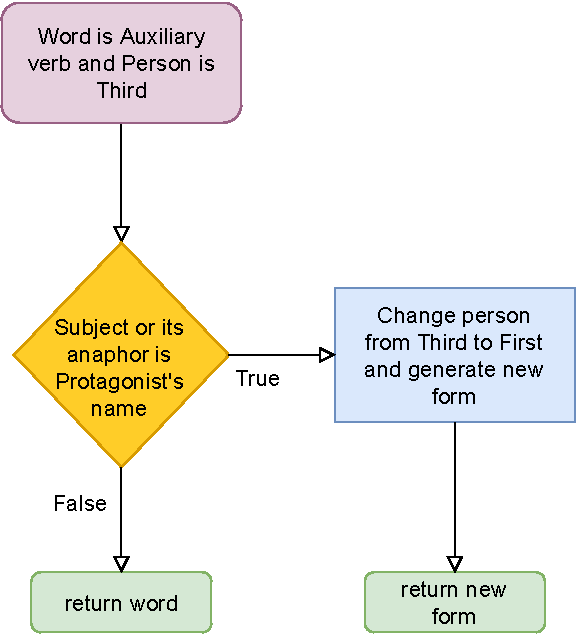
\includegraphics[]{data/Erich-Conditional-Rule.pdf}
\caption{Rule replacing the conditional auxiliars}
\label{fig:erich-conditional-rule}
\end{figure}

\subsection{Auxiliars addition}

I talk about auxiliar deletion in the First-person $\rightarrow$ Third-person conversion section. Naturally, in the opposite direction, the auxiliars need to be added. Thus, the rule considers the participles. For each predicate expressed as a participle, we find the subject. If the subject refers to the protagonist, an auxiliary verb would be added.

Figure \ref{fig:erich-auxverb-rule} illustrates this rule.


\begin{figure}[!htbp]
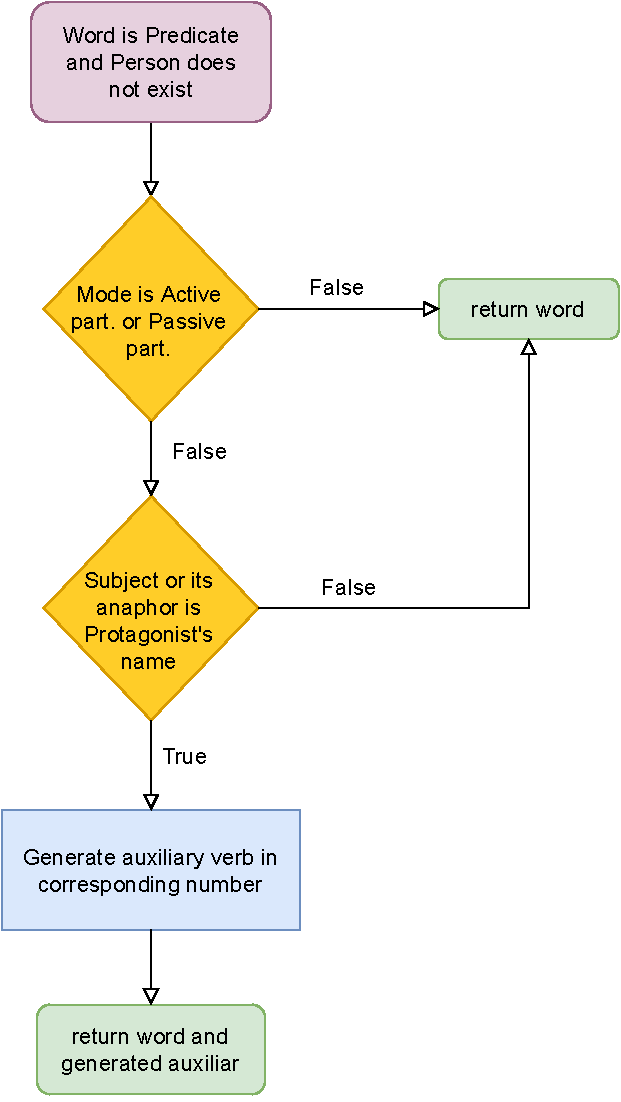
\includegraphics[]{data/Erich-Auxverb-Rule.pdf}
\caption{Rule adding the auxiliars to the sentence}
\label{fig:erich-auxverb-rule}
\end{figure}

\subsection{Personal pronouns}

This rule covers the conversion of personal pronouns. The goal is to replace the pronouns which refer to the protagonist with a personal pronoun in the first person, as shown in the figure \ref{fig:erich-perspron-rule}.

\begin{figure}[!htbp]
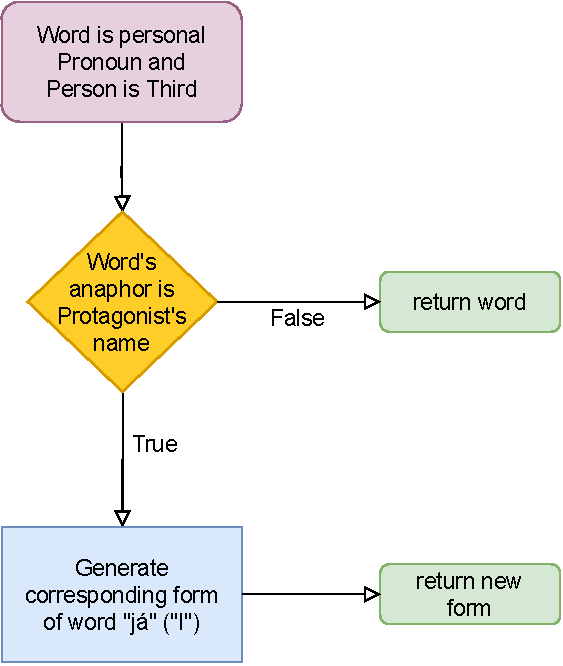
\includegraphics[]{data/Erich-Perspron-Rule.pdf}
\caption{Rule replacing the personal pronouns}
\label{fig:erich-perspron-rule}
\end{figure}

\subsection{Possessive pronouns}

As you can see in figure \ref{fig:erich-posspron-rule}, the process of replacing possessive pronouns is almost the same as the previous one. Nevertheless, finding whom the pronoun refers to is more complicated.

\begin{figure}[!htbp]
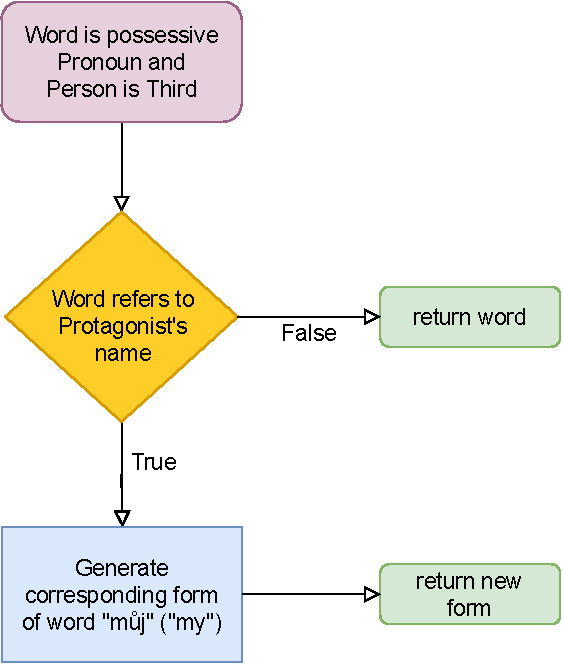
\includegraphics[]{data/Erich-Posspron-Rule.pdf}
\caption{Rule replacing the possessive pronouns}
\label{fig:erich-posspron-rule}
\end{figure}

\subsection{Conjunctions}

The rule is not applied directly to the conjunction but only retrospectively when applying the rule for adding auxiliary verbs, as can be seen in Figure \ref{fig:erich-conjs-rule}.

\begin{figure}[!htbp]
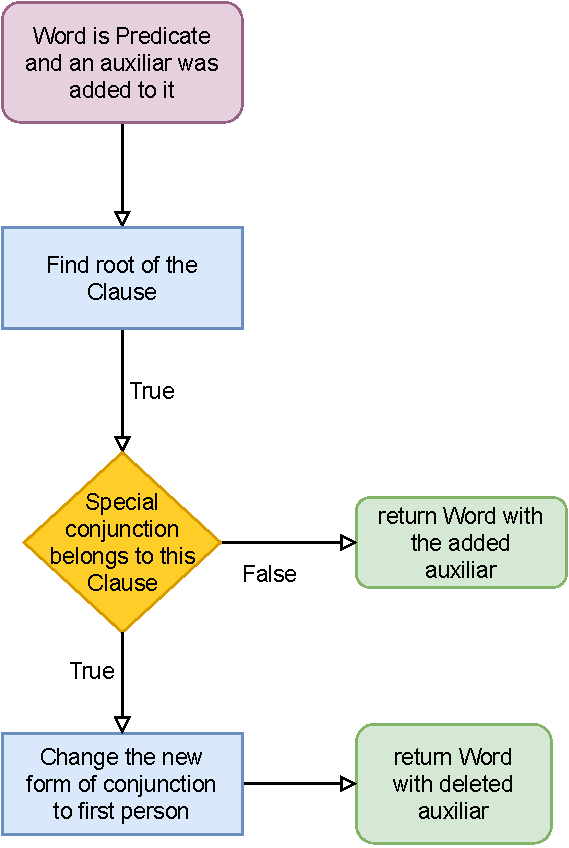
\includegraphics[]{data/Erich-Conjs-Rule.pdf}
\caption{Rule replacing the special conjunctions}
\label{fig:erich-conjs-rule}
\end{figure}


\section{Direct speech}

The last rule is independent of the person, and it covers the processing of direct speech. The simplifying assumption is that the direct speech is in quotes. Therefore, all the text found in quotes should be ignored during the conversion process.

